%%%%%%%%%%%%%%%% NÃO ALTERE O CAMPO ABAIXO 
\documentclass[10pt,twoside,a4paper]{article}
\usepackage[T1]{fontenc}
\usepackage[utf8]{inputenc}
\usepackage[portuges]{babel}
\usepackage[a4paper]{geometry}
\geometry{tmargin=1.2cm,bmargin=1.7cm,lmargin=1.5cm,rmargin=1.5cm}
\usepackage{graphicx}
\usepackage{indentfirst}
\usepackage{subcaption} % figuras lado a lado
\usepackage{booktabs} %tabelas
\usepackage{url}% web links
\usepackage{semat}
\usepackage{lipsum} %Texto automático
\usepackage{amsthm, amsmath, amssymb, wasysym, MnSymbol}
%%%%%%%%%%%%%%%%

%%%%%%%%%%%%%%%% Se necessitar de pacotes adicionais insira abaixo
%\usepackage[•]{•}
%%%%%%%%%%%%%%%%%%%%%%%%%%%%%%%%

%%%%%%%%%%%%%%%%%%
% Evite redefinir ou criar comandos, por exemplo:
% \R=\mathbb{R} ,\newtheorem{teo}{Teorema}, etc
% Isto pode gerar conflito quando os trabalhos forem
% compilados juntos para o caderno de resumos
\newtheorem{theorem}{Teorema}
\newtheorem{proposition}[theorem]{Proposição}
\newtheorem{lemma}[theorem]{Lema}
\newtheorem{definition}[theorem]{Definição}
\newtheorem{corollary}[theorem]{Corolário}
\renewcommand{\qedsymbol}{$\blacksquare$}
\renewcommand{\sin}{{\rm{sen}\hspace{2pt}}}
\renewcommand{\sinh}{{\rm{senh}\hspace{2pt}}}
%%%%%%%%%%%%%%

%%%%%%%%%%% Não altere os comandos abaixo
\newcommand*{\affaddr}[1]{#1} 
\newcommand*{\affmark}[1][*]{\textsuperscript{#1}}
\newcommand*{\email}[1]{\texttt{#1}}
\usepackage{helvet}% Fonte 
\renewcommand{\familydefault}{\sfdefault}% Fonte 
\renewcommand\Authands{ e }
\evento{XVIII Semat e VIII Semest}
\date{02 a 05 de outubro de 2018}
%%%%%%%%%%%%%%%%
% Dados do trabalho
\title{Coloque aqui o título do seu trabalho}
% Autores: o primeiro será, necessariamente, o apresentador do trabalho
\author[1]{\underline{Primeiro Autor Apresentador}\thanks{autor1@ufu.br}}
\author[2]{Segundo Autor\thanks{autor2@unicamp.br}}
\author[1]{Terceiro Autor Orientador\thanks{orientador@ufu.br}}
\affil[1]{FAMAT - Universidade Federal de Uberlândia}
\affil[2]{FEELT - Universidade Federal de Uberlândia}
%palavras-chave: insira até três palavras
\keywords{Palavra um. Palavra dois. Palavra três.}





%Os titulos das seções são apenas exemplos.
%deve-se manter (obrigatoriamente) as seções Resumo e Referências.
%Compilar o arquivo com PDFLatex
%--------------------------------------------------
\begin{document}
\inserirtitulo
\linespread{1.5}% Espaçamento 1.5
%==================================
% RESUMO
%==================================

\section{Resumo}
\lipsum[1] % apague este comando e insira aqui o seu resumo


%==================================
% INTRODUÇÃO
%==================================
\section{Introdução} % apague as linhas abaixo e insira aqui a introdução
\lipsum[2-3] 

Tal resultado pode ser encontrado em \cite{lamport94}.

%==================================
% Primeira Seção
%==================================
\section{Seção Um} % apague as linhas abaixo e insira aqui a primeira seção
\lipsum[7-8]
\begin{theorem}
Este é um exemplo de Teorema
\end{theorem}
\begin{proof}
\lipsum[2]
\end{proof}

%==================================
% Segunda Seção
%==================================
\section{Seção Dois} % apague as linhas abaixo e insira aqui a segunda seção
\lipsum[5]

Verifique a Figura~\ref{fig:distribuicao}.


\begin{figure}[!ht]
\centering
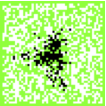
\includegraphics[scale=1.4]{cnmac2}
\caption{Um exemplo de figura.}
\label{fig:distribuicao}
\end{figure}

\lipsum[4]

\begin{proposition}
Este é um exemplo de Proposição
\end{proposition}
\begin{proof}
\lipsum[2]
\end{proof}

\lipsum[3-4]

\begin{figure}[!ht]
\centering
\begin{subfigure}{0.49\textwidth}
\centering
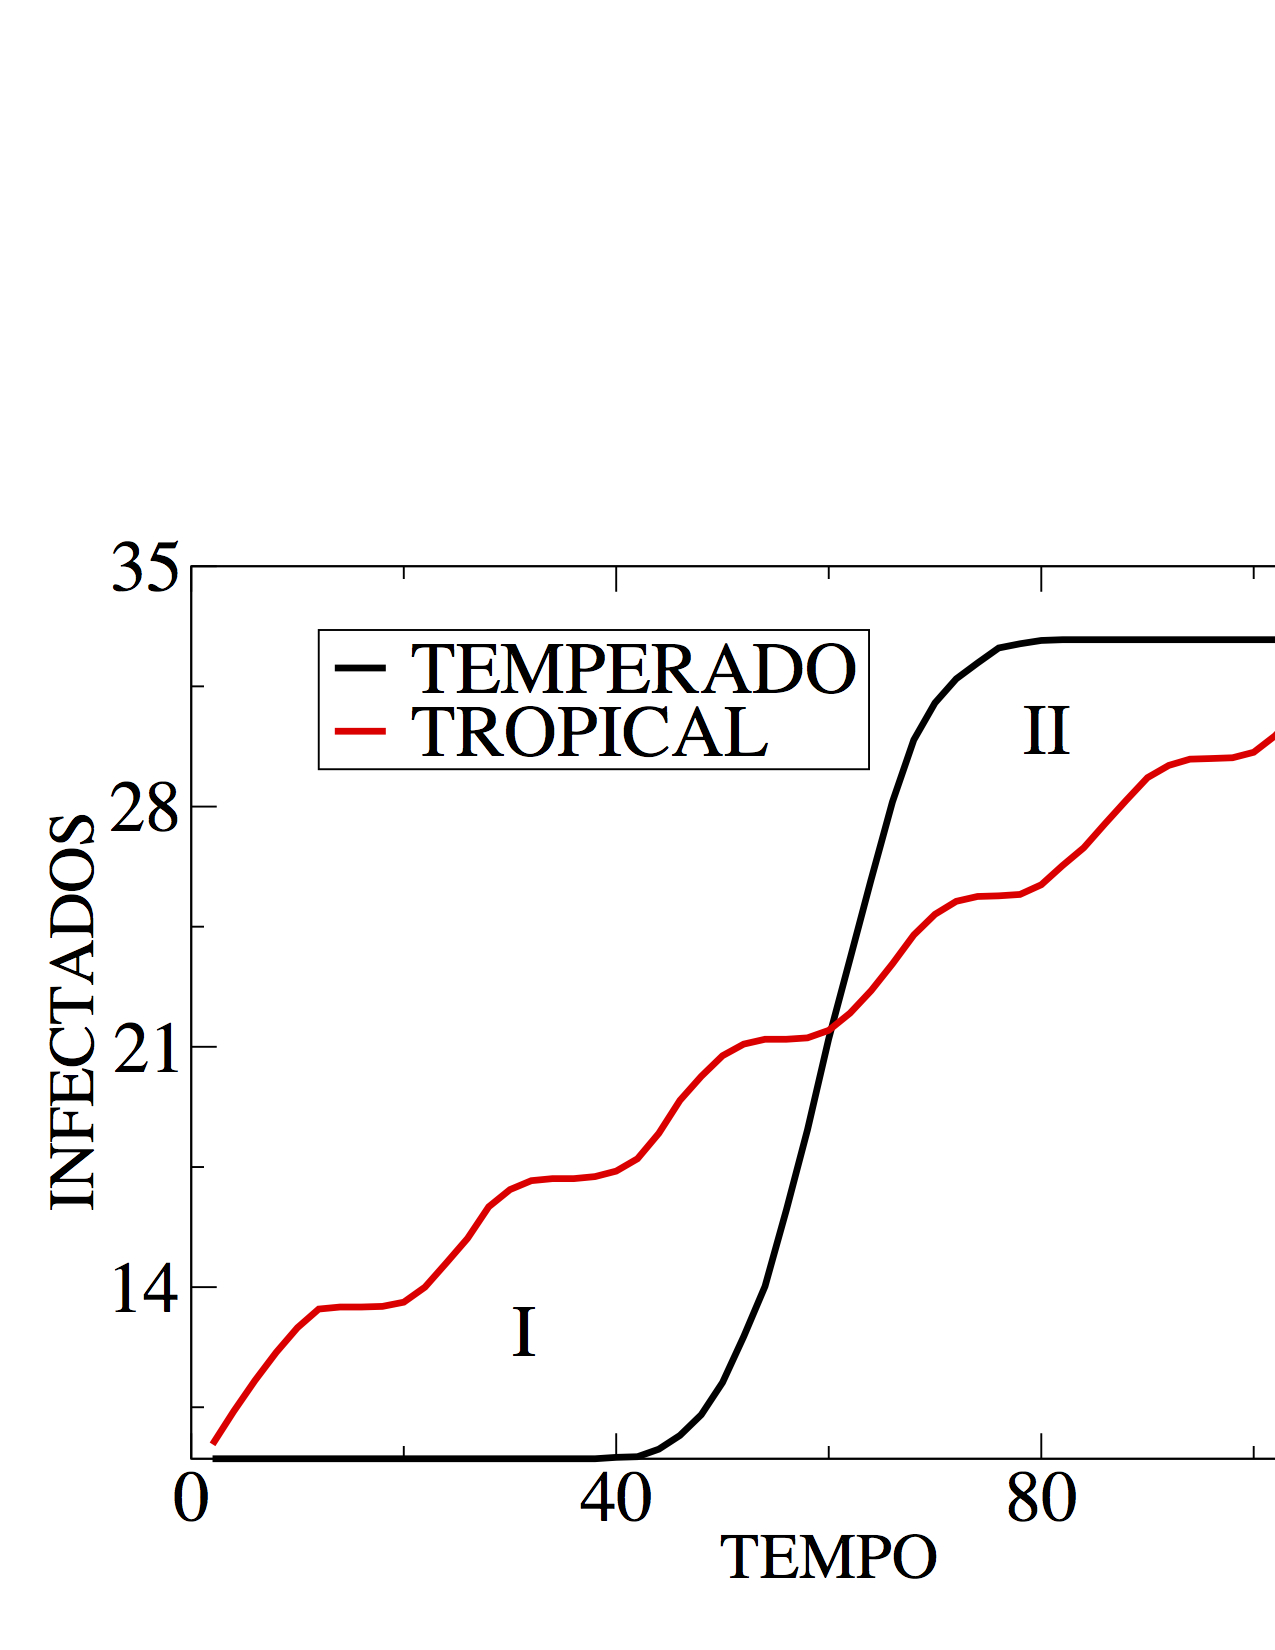
\includegraphics[scale=0.2]{cnmac3}
\caption{Left figure}
\label{fig:left}
\end{subfigure}
\begin{subfigure}{0.49\textwidth}
\centering
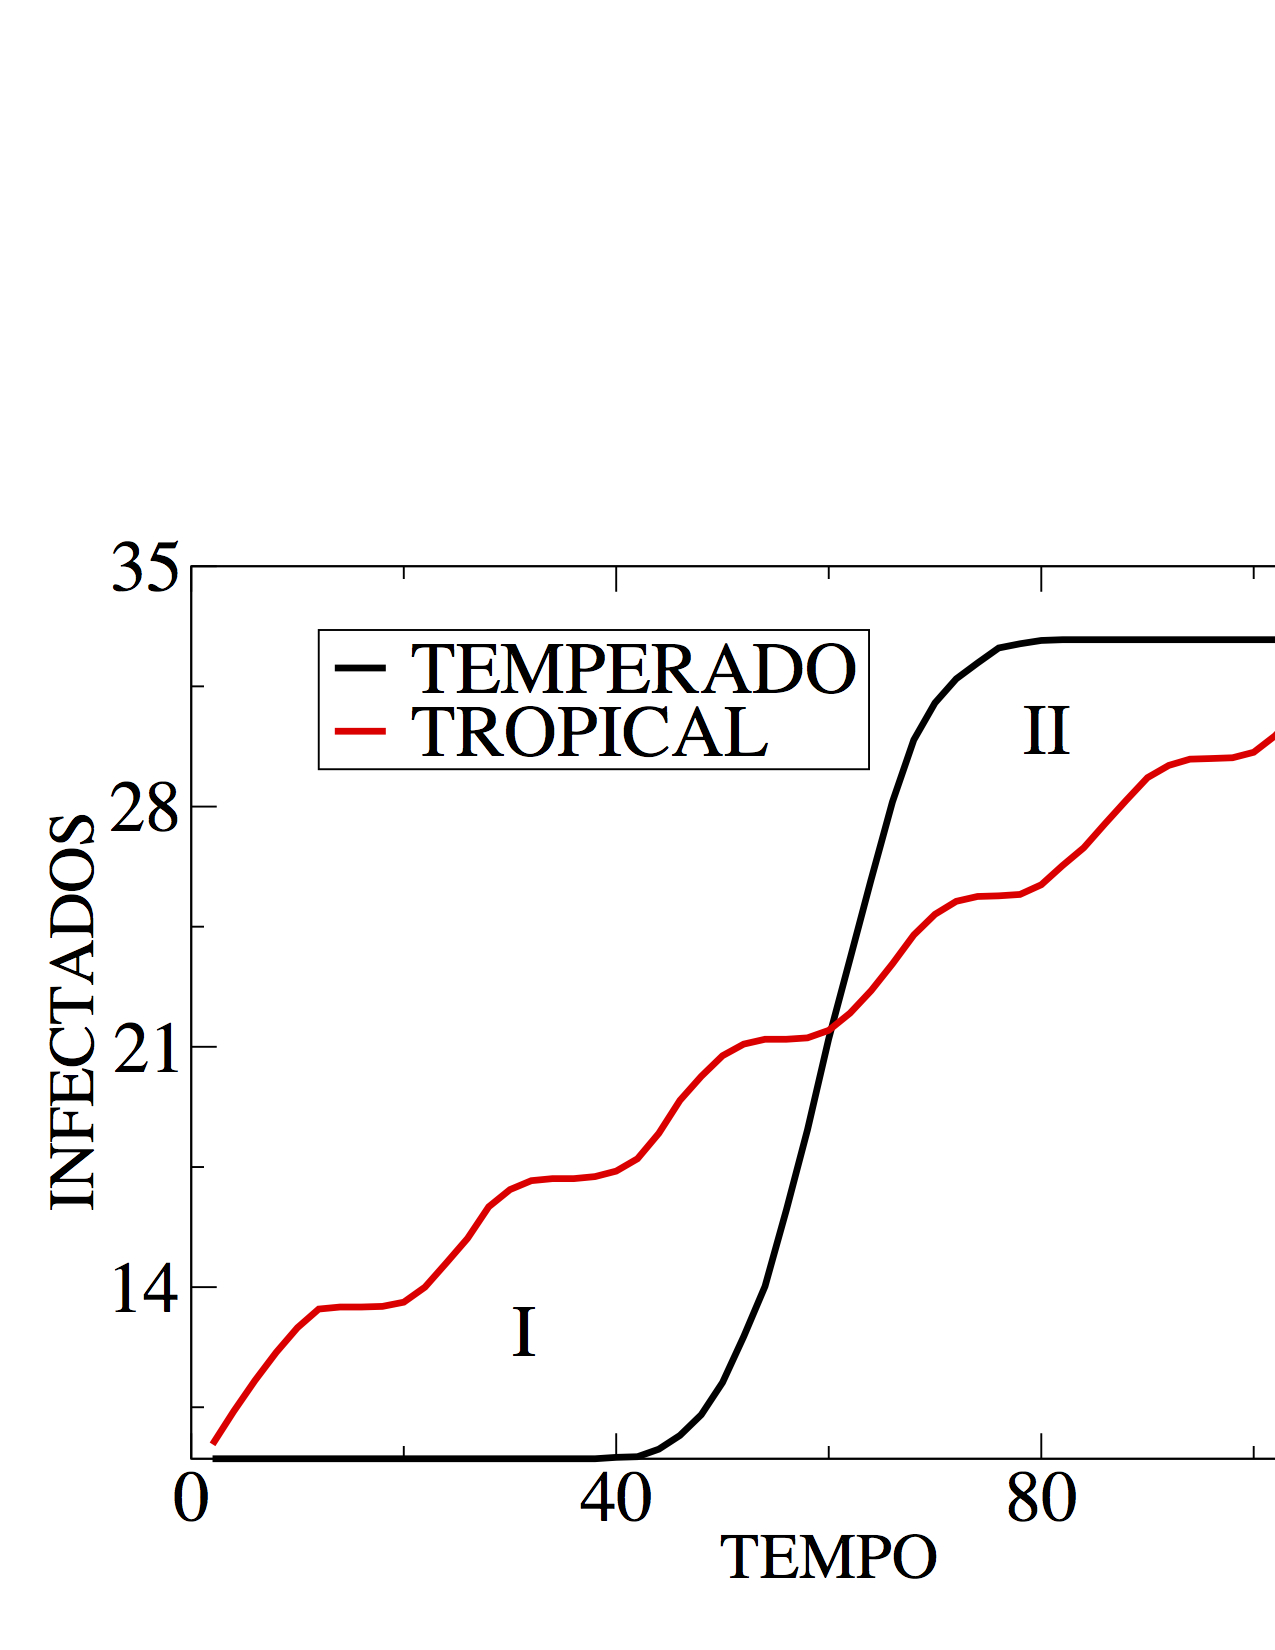
\includegraphics[scale=0.2]{cnmac3}
\caption{Right figure}
\label{fig:right}
\end{subfigure}
\caption{Figuras lado a lado}
\label{fig:combined}
\end{figure}

\lipsum[5]

\begin{center}
Para tabelas, sugerimos a leitura do manual \url{https://www.tug.org/pracjourn/2007-1/mori/mori.pdf}
\end{center}

\begin{table}[h!]
\label{tabela1}
\caption{Maximum  load  and  nominal  tension .}
\centering
\begin{tabular}{clccc}
\toprule
$D$ &               & $P_u$      & $\sigma_N$    \\
(in)&               & (lbs)      & (psi)          \\  \toprule
%
5    & test 1      & 285         & 38.00   \\
& test 2      & 287         & 38.27          \\
& test 3      & 230         & 30.67          \\   \midrule
10   & test 1      & 430         & 28.67   \\
& test 2      & 433         & 28.87          \\
& test 3      & 431         & 28.73          \\    \bottomrule
\end{tabular}
\end{table}



%==================================
% CONCLUSÃO
%==================================
\section{Conclusão} % apague as linhas abaixo e insira aqui a conclusão
\lipsum[8-9]

%==================================
% AGRADECIMENTOS
%==================================
\section{Agradecimentos} % apague as linhas abaixo e insira aqui os agradecimentos
\lipsum[4]


%==================================
% REFERÊNCIAS
%==================================
\begin{thebibliography}{9} % apague as linhas abaixo e insira aqui bibliografia

\bibitem{lamport94}
  Leslie Lamport,
  \emph{\LaTeX: a document preparation system},
  Addison Wesley, Massachusetts,
  2nd edition,
  1994.

\bibitem{pchave2}
  Leslie Lamport,
  \emph{\LaTeX: a document preparation system},
  Addison Wesley, Massachusetts,
  2nd edition,
  1994.

\end{thebibliography}

%--- FIM ---
\end{document}
